% -----------------------------*- LaTeX -*------------------------------
\documentclass[12pt]{report}
\usepackage{scribe_hgen486}
\usepackage{graphicx}
\newcommand{\indep}{\rotatebox[origin=c]{90}{$\models$}}
\begin{document}

\scribe{Joseph Marcus}   % required
\lecturenumber{17}     % required, must be a number
\lecturedate{March 10}    % required, omit year
\lecturer{John Novembre} 

\maketitle

% please leave this comment 
\framebox[.95\textwidth]{\parbox{.93\textwidth}{ {{\bf Note:}} These
lecture notes are still rough, and have only have been mildly
proofread.  }}
\vspace*{.1in}


% feel free to delete content below this line 
% ----------------------------------------------------------------------

\subsection*{Introduction}

Today's lecture introduced undirected probabilistic graphical models and briefly discussed diffusion processes.

\subsection*{Undirected Probabilistic Graphical Models}

\subsubsection*{Review of Directed Graphs}

Recall the canonical directed graph that we have used for numerous examples during lecture (\textit{Figure 1}). We can take advantage of the factorization of directed probabilistic graphical models to efficiently compute the joint distribution of the random variables or various combinations of conditional probabilities. Let $X = \{X_1, X_2, X_3, X_4, X_5, X_6\}$ denote the set of random variables, i.e. nodes, in the graph. We can then write down the probability of $X$ i.e. joint distribution of $X_1, X_2, \dots, X_6$ as:

$$Pr(X) = \prod_{i} Pr(X_i \mid Parents(i))$$ 

\begin{figure}[h!]
\centering
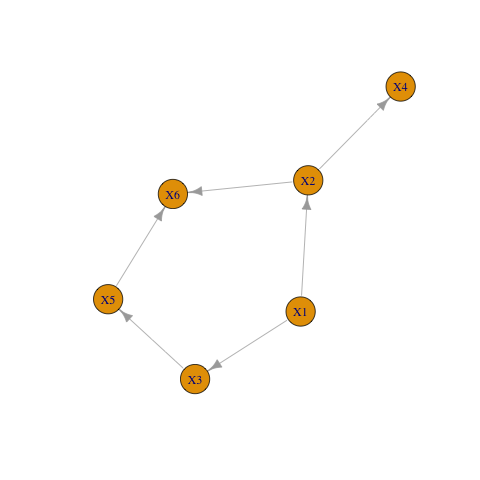
\includegraphics[width=.35\textwidth]{figures/lec17_graph1.png} 
\caption{Directed probabilistic graphical model where each node represents a random variable and edges represent conditional dependencies} \end{figure} 

Where $Parents(i)$ represents the conditioning on the parent nodes of child node $i$. We can use algorithms of the flavor of the Sum-Product algorithm to compute the joint distribution of the above random varibles through the use of message passing functions. For example, we covered Felsenstein's Pruning Algorithm for computing the likelihood of a tree. While the directed probabilistic graph is useful representation of conditional dependencies of random variables there are other graph-based approaches we can take. Specifically we can use an undirected graph structure to represent a probabilistic model. 

\newpage
\subsubsection*{d-separation}

To understand the use of undirected graphs for probabilistic modeling it is helpful to introduce the notion of \textit{d-separation}. Two nodes $X_1$, and $X_2$ are d-separated if when conditioned on a third node they are independent. For example lets take another look at our canonical graph but zoomed in on the sub-graph $\{X_2, X_5, X_6\}$ (\textit{Figure 2}). $X_5$ and $X_2$ are not d-separated because when conditioned on $X_6$ they are not independent. 

\begin{figure}[h!]
\centering
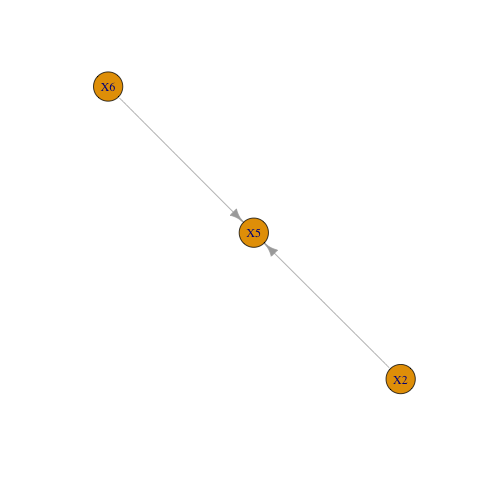
\includegraphics[width=.38\textwidth]{figures/lec17_graph2.png} 
\caption{Sub-graph of the above example to illustrate d-separation} 
\end{figure} 

\newpage

In a undirected graph there is a natural visual interpretation of d-separation. Particularly if every path between node $X_{A}$ and node $X_{B}$ contains $X_{C}$ then $X_{A}$ and $X_{B}$ are d-separated $\equiv X_A \indep X_B \mid X_C$. This can be easily visualized in a undirected graph by tracing the paths between two nodes. It is a helpful exercise to the reader to try to condition on various nodes in the Markov Random Fields below. 

\begin{figure}[h!]
\centering
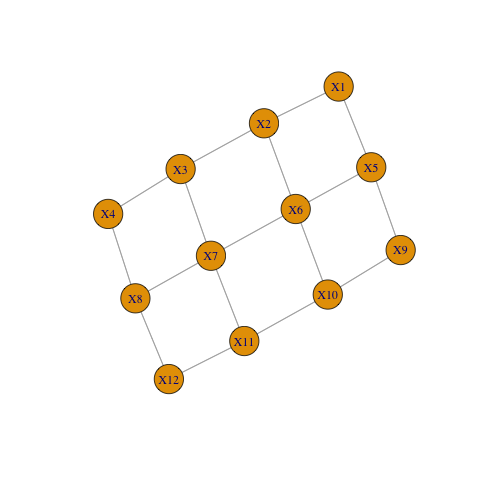
\includegraphics[width=.38\textwidth]{figures/lec17_graph3.png} 
\caption{Markov Random Field Example} 
\end{figure} 

\begin{figure}[h!]
\centering
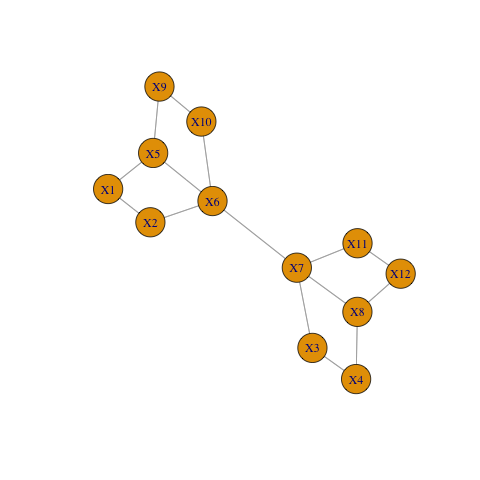
\includegraphics[width=.38\textwidth]{figures/lec17_graph4.png} 
\caption{Markov Random Field Example for d-separation} 
\end{figure} 

\newpage
\subsubsection*{Graph Moralization}

Graph moralization is a term for converting a directed graph into a undirected graph. Every graph has a corresponding undirected graph. If we revisit figure 2 we can perform graph moralization by "marrying" the "un-married" parents and then removing directions on the edges. Specifically we add an edge between $X_2$ and $X_5$ and remove all the directions of edges. Another useful definition is the Markov blanket which is the set of neighbors of a particular node. The Markov blanket helps us consider what random variables to condition on in the Gibbs sampling algorithm i.e. $P(X_i \mid Neighbors(X_i))$. Some useful advantages immediately become clear when using undirected graphs for probabilistic models:

1. We can easily visualize conditional independencies\\ 
2. We no longer need d-separation we can just simply use graph separation\\
3. Makes clear the Markov blanket i.e. what variables that need to be conditioned on in Gibbs sampling

\subsubsection*{Potential Factorization}

We can define a clique of a undirected graph a set of nodes connected to each other. There is an equivalent factorization as we saw in the directed graph setting for undirected graphs. Particularly we can take the product of a potential function for cliques within the graph to compute the joint distribution of the random variables we are modelling:

$$P(X) = \prod_C \Psi_{c}(X_c)$$

Where we define $\Psi(.)$ as a potential function. 

\subsubsection*{Factor Graph}

Another method of computing joint probability distributions on undirected graphs is by defining factor functions between different nodes of a graph. Starting from the top factor graph and going down the column we can write down the joint distribution of random variables of the graph in terms of products of the factor functions (Figure 5):

$$P(X) = f_{1}(X_1, X_3) f_{2}(X_1, X_2) f_{3}(X_2, X_3)$$
$$P(X) = f_{2}(X_1, X_2) f_{1}(X_2, X_3)$$
$$P(X) = f(X_1, X_2, X_3)$$

\newpage

\begin{figure}[h!]
\centering
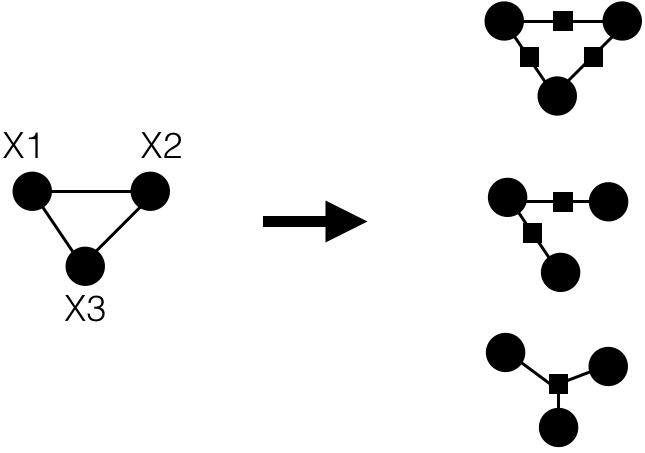
\includegraphics[width=\textwidth]{figures/lec17_factor.png} 
\caption{Factor Graph Example} 
\end{figure} 

\newpage

Factors graphs allow one to deal with more complicated graph structures. One should note that if the factor graph is a tree then the general sum-product algorithm gives efficient computation of all singleton marginals $P(X_i)$ for all $i \in V$ where $V$ is the set of vertices. Also note to look into the junction tree algorithm. 

\subsection*{Diffusion Theory}

Jump processes which include many Markov chains, Poisson processes have low transition probabilities but when transitions occur large changes in state are made. Diffusion processes such as Brownian motion and other Markov chains have high transition probabilities but have when a transition occurs small transitions in state are made. We can model the behavior of diffusion process using second order partial differential equations:

$$P_{t}(x) = P(X(t) = x)$$
$$\frac{\partial P_{t}(x)}{\partial t} = \frac{\partial}{\partial t} [P_{t}(x) M(x)] + \frac{\partial^2}{\partial t^2} [P_{t}(x)M(x)]$$
$$x(t + \delta t) - x(t) = \delta_x$$
$$E[\delta_x] = M(x) \delta t + O(\delta t)$$
$$Var[\delta_x] = V(x) \delta t + O(\delta t)$$

We can use the above diffusion equations to solve for the stationary distributions and transient distributions of a variety of stochastic processes.


\end{document}
